\textbf{\underline{OZ 4 - De wet van Ampère en de wet van Biot-Savart - Oefening 4:}}
\vspace{0.5cm}

Bepaal de grootte, richting en zin van het magnetische veld dat geproduceerd wordt
in het punt $P$ door de stroomvoerende lus.

\begin{center}
    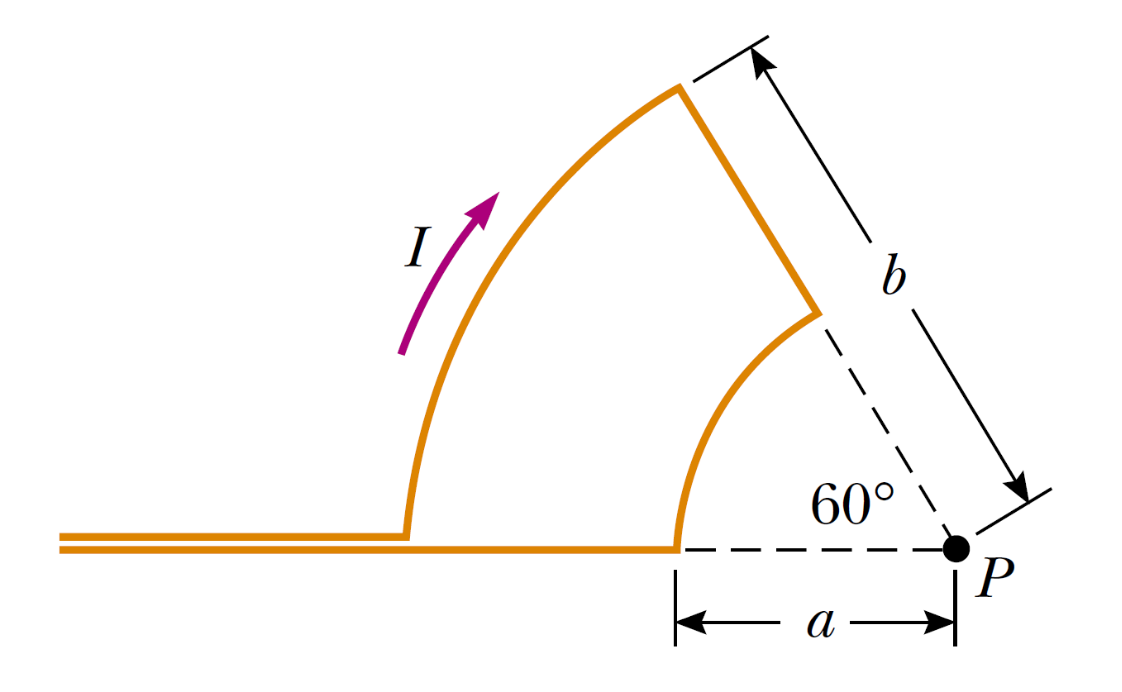
\includegraphics[scale = 0.3]{oz04/resources/Oz4Oef4.png}
\end{center}

% \begin{description}[labelwidth=1.5cm, leftmargin=!]
%     \item[Geg. :]   
%     \item[Gevr. :]  
%     \item[Opl. :]  
% \end{description}

\begin{description}[labelwidth=1.5cm, leftmargin=!]
    \item[Geg. :]  $a$, $b$, $\theta$
    \item[Gevr. :] $\Vec{B}$ ?
    \item[Opl. :]  
    Het magnetisch veld zal bepaald worden door de twee booglengtes. 
    \begin{enumerate}[(a)]
        \item 
        Het magnetische veld door de dichtste booglengte is
        \begin{equation*}
            \Vec{B}_a = \frac{\mu_0I}{4a\pi}\int_0^{\theta}ds \ (\hat{k}) = \frac{\mu_0I\theta}{4a\pi} \ (\hat{k})
        \end{equation*}
        \item 
        Het magnetische veld door de verste booglengte is
        \begin{equation*}
            \Vec{B}_b = \frac{\mu_0I}{4b\pi}\int_0^{\theta}ds \ (-\hat{k}) = \frac{\mu_0I\theta}{4b\pi} \ (-\hat{k})
        \end{equation*}
    \end{enumerate}
    De vectorsom hiervan is dan
    \begin{equation*}
        \Vec{B} = \Vec{B}_a + \Vec{B}_b = \frac{\mu_0I\theta}{4\pi}\left(\frac{1}{a}-\frac{1}{b}\right) \ (\hat{k})
    \end{equation*}
    waarbij $\theta = \dfrac{\pi}{3}$.
\end{description}

\vspace{1cm}